\begin{frame}
	\frametitle{Linguagem}
		\begin{tcolorbox}[colback=blue!5,colframe=blue!40!black,title=Cabaz de Bens]
		\'E composto por quantidades de v\'arios bens. Quando se comparam cabazes, os bens s\~ao os mesmos, mas as quantidades de cada um variam...
	\end{tcolorbox}\pause

	Admitamos dois bens: laranjas ($y$) e bolachas de chocolate ($x$).... ($3,2$) \'e um cabaz composto por por 3 bolachas e 2 laranjas. Gr\'aficamente \'e um ponto do espa\c co ($x,y$)
\end{frame}

\begin{frame}
	\begin{center}
		\begin{tikzpicture}
			\draw[->] (-0.1,0) -- (4.1,0) node[below right] {$x$ bolachas};
			\draw[->] (0,-0.1) -- (0,4.1) node[above left] {$y$ laranjas};

			\draw[dashed] (3,0) node[below]{3} -- (3,2) node[blue,circle,fill,inner sep=2pt]{} -- (0,2) node[left]{2};
		\end{tikzpicture}
	\end{center}
\end{frame}

\begin{frame}
	\frametitle{Conjunto das possibilidades de Consumo}

	\begin{itemize}
		\item \'E o conjunto de todos os cabazes que podem ser adquiridos com um dado or\c camento.
		\item O conjunto de cabazes cuja despesa esgota o or\c camento designa-se ``Restri\c c\~ao Or\c camental''
	\end{itemize}

\end{frame}

\begin{frame}
	\frametitle{Problema do Consumidor}
	De entre os cabazes dispon\'iveis no Espa\c co das Possibilidades de Consumo, encontrar a escolha \'optima, dadas as vari\'aveis ex\'ogenas:\pause

	\vspace{0.2cm}

	\begin{itemize}
		\item Or\c camento ($W$)\pause
		\item Pre\c cos de mercado ($p_x,p_y$)\pause
	\end{itemize}
	\vspace{0.4cm}

	O consumidor ir\'a portanto, decidir o valor para as vari\'aveis end\'ogena, $X$ e $Y$, as suas vari\'aveis de decis\~ao!
\end{frame}

\begin{frame}
	\frametitle{Restri\c c\~ao Or\c camental}
	$$X p_x + Y p_y = W$$
	\euro 10 para gastar em bolachas e laranjas. Cada laranja custa 10 c\^entimos, cada bolacha custa 25 c\^entimos
	
	
	A restri\c c\~ao or\c camental ser\'a... \pause

	$$0.25 X + 0.1 Y = 10$$

\end{frame}

\begin{frame}
	\frametitle{Restri\c c\~ao Or\c camental}

	\begin{center}
		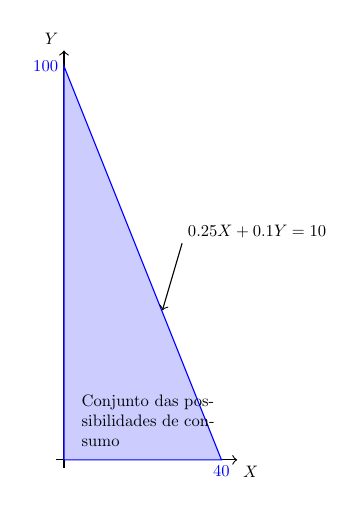
\begin{tikzpicture}[
				every node/.style={scale=0.6},
			]

			\draw[->] (-0.1,0) -- (2.2,0)node[below right]{$X$};
			\draw[->] (0,-0.1) -- (0,5.2)node[above left]{$Y$};

			\draw[blue,fill=blue!20] (0,0) -- (0,5) node[left]{$100$} -- (2,0) node[below]{$40$} -- (0,0);
			
			\draw[->] (1.5,2.75)node[above right]{$0.25X+0.1Y=10$} -- (1.25,1.9);
			\draw (0.15,0.1) node[above right, text width = 0.25\textwidth]{Conjunto das possibilidades de consumo};

		\end{tikzpicture}
	\end{center}
	A Restri\c c\~ao Or\c camental tamb\'em pode ser descrita, neste gr\'afico como $Y = 100 - 2.5X$
\end{frame}

\begin{frame}
	\frametitle{Restri\c c\~ao Or\c camental- Altera\c c\~ao do pre\c co}

	\begin{center}
		\def\w{5}
		\def\dw{1.5}
		\def\px{3}
		\def\py{3.5}
		\def\pxx{4}
		\def\pyy{2.5}
		\begin{tikzpicture}[
				scale = 1.5,
				every node/.style={scale=1},
				declare function = {bc1(\x) = (\w/\py) - (\px/\py)*\x;},
				declare function = {bc2(\x) = (\w/\py) - (\pxx/\py)*\x;},
				declare function = {bc3(\x) = (\w/\pyy) - (\px/\pyy)*\x;}
			]

			\draw[->] (-0.1,0) -- ({\w/2},0)node[below right]{$X$};
			\draw[->] (0,-0.1) -- (0,{\w/2})node[above left]{$Y$};
			
			\only<1>{
				\draw[] (0,{bc1(0)}) node[left] {$\frac{W}{p_Y}$} -- ({\w/\px},{bc1(\w/\px)}) node[below] {$\frac{W}{p_X}$};
				\draw[->] (1,{bc1(1)}) -- (1.5,{bc1(1)+0.55}) node[right]{$Xp_x+Yp_y=W$};
			}

			\only<2>{
				\draw[dashed,gray] (0,{bc1(0)}) node[left] {$\frac{W}{p_Y}$} -- ({\w/\px},{bc1(\w/\px)}) node[below] {$\frac{W}{p_X}$};
				\draw[] (0,{bc2(0)}) node[left] {$\frac{W}{p_Y}$} -- ({\w/\pxx},{bc2(\w/\pxx)}) node[below] {$\frac{W}{\hat{p}_X}$};
				\draw[->] (1,{bc2(1)}) -- (1.5,{bc1(1)+0.55}) node[above right]{Aumento de $p_x$ a $\hat{p}_x$};
			}

			\only<3>{
				\draw[] (0,{bc1(0)}) node[left] {$\frac{W}{p_Y}$} -- ({\w/\px},{bc1(\w/\px)}) node[below] {$\frac{W}{p_X}$};
				\draw[->] (1,{bc1(1)}) -- (1.5,{bc1(1)+0.55}) node[right]{$Xp_x+Yp_y=W$};
			}

			\only<4>{
				\draw[dashed,gray] (0,{bc1(0)}) node[left] {$\frac{W}{p_Y}$} -- ({\w/\px},{bc1(\w/\px)}) node[below] {$\frac{W}{p_X}$};
				\draw[] (0,{bc3(0)}) node[left] {$\frac{W}{\hat{p}_Y}$} -- ({\w/\px},{bc3(\w/\px)}) node[below] {$\frac{W}{p_X}$};
				\draw[->] (1,{bc3(1)}) -- (1.5,{bc3(1)+0.55}) node[above right]{Diminui\c c\~ao de $p_y$ a $\hat{p}_y$};
			}

			\onslide<5->{
				\draw[] (0,{bc1(0)}) node[left] {$\frac{W}{p_Y}$} -- ({\w/\px},{bc1(\w/\px)}) node[below] {$\frac{W}{p_X}$};
			}

			\only<6>{
				\draw[red,domain=0:((\w-\dw)/\px),variable=\x] plot (\x,{bc1(\x)-(\dw/\py)});
				\draw[red] (1.5,{bc1(1)+0.55}) node[above right]{Diminui\c c\~ao de $W$};
			}

			\only<7>{
				\draw[red,domain=0:((\w+\dw)/\px),variable=\x] plot (\x,{bc1(\x)+(\dw/\py)});
				\draw[red] (1.5,{bc1(1)+0.55}) node[above right]{Aumento de $W$};
			}			

		\end{tikzpicture}
	\end{center}
\end{frame}

\begin{frame}
	\frametitle{Declive da Restri\c c\~ao Or\c camental}
	\begin{align*}
		X P_x + Y p_y = W \quad \Leftrightarrow \quad Y = {\color{red}\frac{W}{p_y}} - {\color{blue}\frac{p_x}{p_y}}X
	\end{align*}

	\begin{itemize}
		\item $\frac{W}{p_y}$: {\color{red}Ordenada na Origem}
		\item $-\frac{p_x}{p_y}$: {\color{blue}Declive}
	\end{itemize}

	$$0.25X + 0.1Y = 10 \quad \Leftrightarrow \quad Y = {\color{red}100} - {\color{blue}2.5} X$$
\end{frame}


\begin{frame}
	\frametitle{Escolha \'optima do consumidor}
	Do conjunto das possibilidades de consumo, escolher o cabaz \'optimo ($x,y$) em fun\c c\~ao de:\pause
	\vspace{0.2cm}
	\begin{itemize}
		\item Vari\'aveis ex\'ogenas (pre\c cos, rendimento)
		\item Prefer\^encias...
			\begin{itemize}
				\item Axiom\'atica de prefer\^encias
			\end{itemize}
	\end{itemize}
\end{frame}

\begin{frame}
	\frametitle{Axiom\'atica de Prefer\^encias}
	\begin{itemize}
		\item \textbf{Desejabilidade} ou \textbf{N\~ao Saciedade}: Consumir mais, \'e melhor
	\end{itemize}

	Ent\~ao, por exemplo, o consumidor vai preferir o cabaz $A=(25,30)$ ao cabaz $B=(20,20)$ simplesmente porque o cabaz $A$ cont\'em mais quantidade (para ambos bens) do que o cabaz $B$.

\end{frame}

\begin{frame}
	\frametitle{Desejabilidade}
	\begin{center}
		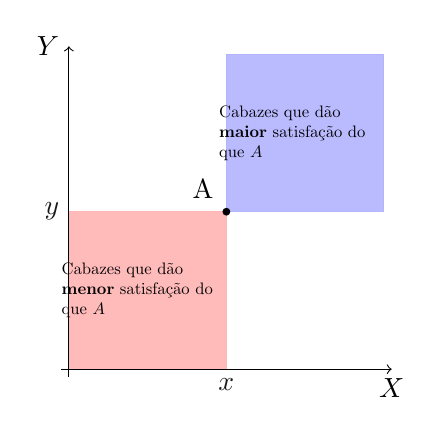
\begin{tikzpicture}
			\draw[fill,red!30,opacity=0.9] (0,0) -- (0,2) node[black,left] {$y$} -- (2,2) -- (2,0) node[black,below]{$x$} -- (0,0);
			\draw[fill,blue!30,opacity=0.9] (2,2) -- (4,2) -- (4,4) -- (2,4) -- (2,2);

			\draw[->] (-0.1,0) -- (4.1,0) node[below]{$X$};
			\draw[->] (0,-0.1) -- (0,4.1) node[left]{$Y$};

			\draw(2,2) node[circle,fill,inner sep=1pt,label = above left:A]{};
			\draw(1,1) node[text width = 0.3\textwidth, scale = 0.6] {Cabazes que d\~ao \textbf{menor} satisfa\c c\~ao do que $A$};
			\draw(3,3) node[text width = 0.3\textwidth, scale = 0.6] {Cabazes que d\~ao \textbf{maior} satisfa\c c\~ao do que $A$};
		\end{tikzpicture}
	\end{center}

\end{frame}

\begin{frame}
	\frametitle{Axiom\'atica de Prefer\^encias}
	E se um cabaz cont\'em mais de um bem e menos do outro?! Qual o preferido? (20,30) ou (30,20)?!?
	\vspace{0.2cm}
	\begin{itemize}
		\item<1-> \'E preciso saber quais s\~ao os cabazes indiferentes entre si...
		\item<2-> Quantas laranjas est\'a o consumidor disposto a abdicar, para ter mais uma bolacha de chocolate e ficar indiferente?
		\begin{itemize}
			\item<3-> A resposta n\~ao depende do que pode comprar dadas as suas possibilidades de consmo, mas apenas das prefer\^encias.
		\end{itemize}
	\end{itemize}

\end{frame}

\begin{frame}
	\frametitle{Curva de Indiferen\c ca}
	\begin{tcolorbox}[title=Curva de indiferen\c ca]
		Conjunto dos cabazes indiferentes entre si!
	\end{tcolorbox}

	\begin{itemize}
		\item<2-> Devido \`a hip\'otese de desejabilidade, os cabazes indiferentes entre si n\~ao podem conter mais quantidade de ambos os bens, nem podem conter menos quantidade de ambos os bens: t\^em de conter sempre mais de um e menos do outro.
		\item<3-> No espa\c co $XY$, a curva de indiferen\c ca tem de ter inclina\c c\~ao negativa!
	\end{itemize}

\end{frame}

\begin{frame}
	\frametitle{Curva de Indiferen\c ca}
	\begin{center}
		\def\a{1/2}
		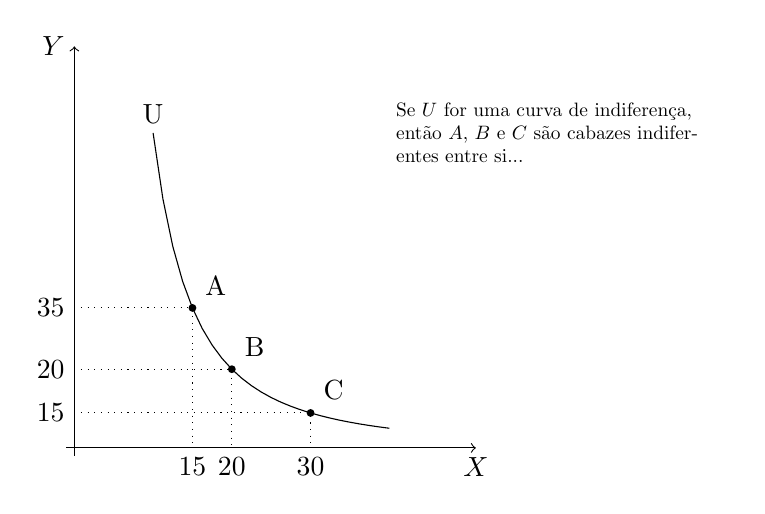
\begin{tikzpicture}[
			scale = 1,
			declare function = {i(\x) = (1/(\x^\a))^(1/(1-\a));},
		]

		\draw[->] (0,-0.1) -- (0,5.1) node[left]{$Y$};
		\draw[->] (-0.1,0) -- (5.1,0) node[below]{$X$};

		\draw[domain=1:4,variable=\x] plot (\x,{i(\x)});

		\draw[dotted] (0,{i(1.5)}) node[left] {35} -- (1.5,{i(1.5)}) node[circle,fill,inner sep=1pt,label = above right:A]{} -- (1.5,0)node[below] {15};
		\draw[dotted] (0,{i(2)}) node[left] {20} -- (2,{i(2)}) node[circle,fill,inner sep=1pt,label = above right:B]{} -- (2,0)node[below] {20};
		\draw[dotted] (0,{i(3)}) node[left] {15} -- (3,{i(3)}) node[circle,fill,inner sep=1pt,label = above right:C]{} -- (3,0)node[below] {30};

		\draw(1,{i(1)}) node[above]{U};

		\draw(4,4) node[right,text width = 0.5\textwidth, scale = 0.7] {Se $U$ for uma curva de indiferen\c ca, ent\~ao $A$, $B$ e $C$ s\~ao cabazes indiferentes entre si...};

		\end{tikzpicture}
	\end{center}
\end{frame}